\begin{savequote}
\quoteperson{They can't keep this level of graphics up for much longer!
We used to be lucky if we only got three shades of grey, let alone any 
real colours!}{Cranky Kong}
\end{savequote}

\chapter{Hardware Assisted Geometric Algebra on the GPU}
\label{chap:gpu}

In this chapter we explore how the \emph{Graphics Processing
Units} (GPUs) in modern consumer-level graphics cards can be
used to perform Geometric Algebra computations faster than a 
typical single-core CPU.

\section{An Overview of GPU Architecture}

\begin{figure}
\centering
\includegraphics[width=0.9\textwidth]{gpu_architecture}
\caption{\label{fig:gpu_architecture}%
  A simplified block diagram of a typical GPU.}
\end{figure}

The GPU in a graphics card is not designed for general purpose 
computing. It is designed, not surprisingly, to perform the
sort of operations useful for graphics rendering. Figure
\ref{fig:gpu_architecture} shows a simplified block diagram of
a typical GPU.

In a traditional fixed-function GPU the CPU uploads, over the AGP
bus, a set of vertices, texture maps and some state information. The
state includes projection and view matrices, clipping planes, 
lighting models, etc. The vertex list and texture maps (if present) 
are then stored in some on-card memory.

On the card there exists a number of rendering pipelines, each of which
can be run in parallel to increase throughput. The pipeline consists
of a \emph{vertex shader} which fetches triplets of vertices from
the vertex memory, transforms them using the current projection and 
view matrices, performs any clipping and sends them to the rasteriser.

The rasteriser takes triplets of screen co-ordinate vertices, forms
a triangle from them and outputs a set of pixel positions which form
render the triangle along with depth information and interpolated texture
co-ordinates. 

The fragment shader takes these pixel positions and, using the texture maps
stored in texture memory along with appropriate state information calculates
the colour of the pixel after all lighting, etc. is performed. The shaded pixel
is then sent to the screen.

In reality the rendering stage is split at the rasteriser allowing for differing
numbers of vertex and fragment shaders but for the purposes of GPU programming
one can view the shaders as being within the same pipeline.

In modern programmable GPUs both the vertex and fragment shaders are fully 
programmable allowing different per-vertex and per-pixel transformation
and shading that is allowed in the traditional fixed-function pipeline.

Each shader is, in effect, an efficient vector processor and, on modern 
graphics cards, there are a number working in parallel. To perform
general purpose computation on the GPU we must find ways of modifying our
algorithms to fit this model.

\section{GPU Programming Methods}

\subsection{DirectX shader language}

Microsoft's DirectX\cite{GPU:DirectX} is a graphics programming API for
Windows and, to some extent, the Microsoft XBox gaming platform. As part of
the API it specifies a generic shading language\cite{GPU:DirectXShadingLanguage}
which abstracts the vertex and fragment shaders. Each version of DirectX
specifies a minimum set of shader capabilities which \emph{must} be supported by a 
card claiming compatibility with that level of the API. Consequently a shader written in
DirectX's shading language is portable across all cards which support that level
of the API. A disadvantage of DirectX is that it doesn't expose any functionality
beyond the specified minimum and it is not portable across operating systems.

\subsection{OpenGL shader language}

OpenGL\cite{GPU:OpenGLSpec} is a cross-platform C-based graphics API. 
It is the \emph{de facto} standard API for non-Windows platforms and
is well supported on Windows platforms by both ATI and nVidia, the dominant
vendors at the time of writing. 

The OpenGL 2.0 specification\cite{GPU:OpenGL2Overview} proposed by 3DLabs
includes a hardware agnostic shading language\cite{GPU:OpenGLShadingLanguage}
known as \emph{GL Shading Language} (GLSL) which provides a similar level
of functionality to that exposed in DirectX. 

Currently few hardware vendors support OpenGL 2.0 --- at the time of writing
nVidia was the only mainstream vendor to provide support in their
consumer-level hardware\cite{nvidia:7664relnotes}.

OpenGL 1.4 and below provide support for programmable shaders via a set of per-vendor
extensions. Unfortunately these require programming the GPU in a variety of
assembly languages and vary between different GPUs.

\subsection{The Cg toolkit from nVidia}

Both the OpenGL and DirectX shading languages have a number of disadvantages
from the point of view of research. The OpenGL shading language, whilst being
high-level and convenient to program in, is not widely available. The
DirectX toolkit provides only a `lowest common denominator' shading language,
it is not particularly high-level and is, for all intents and purposes, limited
to the Microsoft Windows operating systems. 

An attempt to bridge these gaps is the Cg toolkit\cite{nvidia:cgtoolkit} from nVidia.
It provides a high-level C-like shading language which may be compiled at run-time or
ahead of time into either DirectX shading language or the myriad of OpenGL extensions
which exist for accessing the programmable shaders. 

Along with these advantages is the `future-proof' nature of Cg. The core Cg language
is easily extended via so-called `profiles'. These either restrict the language to
correspond to the capabilities of particular GPUs or add more features to expose
new GPU abilities. As an example in figure \ref{fig:gpu_architecture} it was implied
that the vertex shader cannot access the texture-map memory. This was true
of older cards but the latest generation of nVidia cards can
access texture maps from within the vertex shader\cite{nvidia:sm3unleashed}. Adding this
capability to Cg was simply a case of releasing a new profile where texture-map related
parts of the language were now available from within both shaders. Older shaders
would still work however and the presence of this capability could be queried
at run-time.

Because of these advantages it was decided to use Cg as the basis for the GPU
computing research. None of the techniques described below require it as they
can all be re-structured to use alternate APIs.

\section{A Cg Implementation of Generator Exponentiation}

\begin{figure}[p]
\centering
\scalebox{0.8}{
\begin{minipage}{0.8\textwidth}
\singlespacing
\lstinputlisting[language=c]{rotor_tools.cg}
\hrule
\lstinputlisting[language=c]{rotor_tools.h}
\end{minipage}}
\caption{\label{fig:rotortools}The Cg and C interfaces for dealing with rotors and
  exponentiated generators.}
\end{figure}

In order to integrate the GA interpolation scheme described in the previous 
chapter into the GPU graphics pipeline it had to be re-cast into the 
mathematical language of the GPU. Graphics cards are optimised for 
linear algebra on 4-dimensional vectors and $4\times4$ matrices, reflecting
the dominant language used in graphics. 

It was decided to abstract away the GA method and represent rotors and
generators as sets of vectors. The Cg interface, and corresponding CPU-side C
interface, used is shown in figure \ref{fig:rotortools}. The required GA
operations for rotor exponentiation and application ($X \mapsto RX\tilde{R}$)
were expanded out in terms of basis components and implemented
directly in Cg. The routines could now be used as a `black-box' by the GPU 
programmer. Indeed no GA knowledge was required for their use, merely that one
applies rotors to points to transform them, one can convert generators into
rotors and generators may be linearly interpolated.

A more general GA-solution, such as {\tt libcga}, was impractical given the
current space constraints on Cg programs although future GPUs may provide
enough space to make such a library feasible.

\section{Mesh Deformation}

In this section we shall give an example of a vertex shader that uses GA to
perform mesh deformation. The deformation scheme given is a simple application
of Geometric Algebra but nicely shows the applicability of GA
to a wide variety of problems. The method developed has a number of nice 
properties but should be viewed as an illustration of the power of GA
algorithms when implemented on the GPU rather than as a deformation scheme
in its own right.

\subsection{Method}

We shall now present a GA-based mesh deformation scheme suitable for
implementation on a GPU. In this scheme we start with
an existing mesh and set of key rotors, $\left\{ R_1, R_2, \cdots, R_k \right\}$,
which we wish to use to deform the mesh. Our scheme seeks to find some automatic
method of representing each point on the mesh as some function of the key
rotors; changing the key rotors will then lead to a deformation of the mesh. Desirable
properties include smoothness, small changes in the rotors lead to small changes
in the mesh, and to be intuitive, changes in the rotors should produce changes
in the mesh which a user, ignorant of the method, would expect.

\begin{figure}
\centering
\includegraphics[width=0.8\textwidth]{assignment_scheme}
\caption{\label{fig:assignment_scheme}Representing a point, $P_i$, on a mesh as
a rotor, $R_i$, and displacement, $p_i$, given a set of key rotors, 
  $\left\{R_1, R_2\right\}$.}
\end{figure}

Our assignment scheme is illustrated in figure \ref{fig:assignment_scheme}.
Firstly we form a set of generators, $\left\{B_1, B_2, \cdots, B_k\right\}$,
such that
\[
\left\{ R_1, R_2, \cdots, R_k \right\} \equiv \left\{\exp(B_1), \exp(B_2),
        \cdots, \exp(B_k)\right\}.
\]
We also find the image of the origin, $O_k = R_k\bar{n}\tilde{R}_k$, for 
each key-rotor. For each point-representation on the mesh, $P_i$, we find the Euclidean
distance from it to the image of the origin in each key-rotor,
\[
\label{eqn:dki}
d_{k,i} = \sqrt{-2O_k \cdot P_i}.
\]
We then form a rotor, $R_i$, for each point on the mesh as a weighted sum of the
key-rotors,
\[
R_i = \exp\left(\frac{\sum^{k}_1 w_i(d_{k,i}) B_i}{\sum^{k}_1 w_i(d_{k,i})}\right)
\]
where $w_i(d)$ is a function which defines the relative weights of each rotor depending
on its proximity to the mesh point. One might choose a relatively simple weight function
\[
w_i(d) = \frac{1}{d + \epsilon}
\]
where $\epsilon$ is a small value to avoid a singularity when the key-rotor and mesh
intersect. In our implementation we wished to have key-rotors with varying degrees of 
influence. This was accomplished by using a Gaussian weight function,
\[
w_i(d) = \exp\left(-\frac{d^2}{\sigma_i^2}\right)
\]
with $\sigma_i$ giving the radius of influence of a particular key-rotor.

Finally we find a point, $p_i$, which is transformed by $R_i$ to coincide
with $P_i$,
\[
(R_i p_i \tilde{R}_i) \cdot P_i = 0
\]
which may be found by simply applying the reversal of $R_i$ to $P_i$
\[
p_i = \tilde{R}_i P_i R_i.
\]
The point $P_i$ is now stored in memory as a set of $d_{k,i}$ for each
key-rotor and the point $p_i$.

Our deformation procedure is now simple. Given a new set of key-rotors,
$\left\{ R'_1, R'_2, \cdots, R'_k \right\}$, and a corresponding set of
generators, $\left\{B'_1, B'_2, \cdots, B'_k\right\}$, we can form the deformed
mesh point $P'_i$ given the previously calculated $d_{k,i}$ and $p_i$ as
\begin{align}
R'_i &= 
\exp\left(\frac{\sum^{k}_1 w_i(d_{k,i}) B'_i}{\sum^{k}_1 w_i(d_{k,i})}\right) \label{eqn:summation} \\
P'_i &= R'_i p_i \tilde{R}'_i.
\end{align}
It is easy to show by direct substitution that for $R'_k = R_k$ this 
reduces to $P'_i = P_i$ as would be expected.

\subsection{GPU-based implementation}

Since the GPU distinguishes between global state and per-vertex information we
must decide what information needs to be given to the GPU and how. In our mesh
deformation example we need the key-rotors which are part of the global state
and, for each mesh point, the vector $p_i$ and set of distances $d_{k,i}$.

In OpenGL each vertex has at least a three-dimensional position vector associated 
with it and may have a normal vector. In addition there are a number of 
texture co-ordinates which may be associated with each vertex. In our implementation
the values of $w(d_{k,i})$ will be stored into the texture co-ordinates. The weight
function is pre-computed to save time.

\begin{figure}[p]
\centering
\scalebox{0.8}{
\begin{minipage}{\textwidth}
\singlespacing
\lstinputlisting[language=c]{vertex_shader.cg}
\end{minipage}}
\caption{\label{fig:meshshader}The vertex shader used to perform GA-based mesh
deformation.}
\end{figure}

Figure \ref{fig:meshshader} gives the vertex shader used to perform mesh deformation in
this example. Line 2 includes the standard set of rotor manipulation functions which
were described above. 
%For the moment it is sufficient to note that generators are
%stored as a pair of 3-vectors, giving 6 components in all, and rotors are stored as a
%pair of 4-vectors, giving 8 components.

The generators associated with the key rotors are passed in the state array {\tt generators[][]}
and are constant for a particular scene. Lines 32 to 39 perform the summation in 
equation \ref{eqn:summation} and line 41 uses the function {\tt exp\_generator()} to 
form $R'_i$. Line 42 applies $R'_i$ to the point $p_i$ and the remainder of the shader
is boilerplate code to project into screen-space and perform a simple lighting calculation.

\begin{fancyalg}
\begin{algorithmic}[1]
\REQUIRE{$P_i$, the null-vector representation of mesh vertex $i$.}
\REQUIRE{$\mathcal{B} \equiv \{B_1, B_2, \cdots, B_k, \cdots \}$,
  the set of key-rotor generators.}
\STATE $w_{\mathrm{sum}} := 0$
\FOR{$k := 1$ to $n(\mathcal{B})$}
\STATE $R := \exp(B_k)$
\STATE $O := R\bar{n}\tilde{R}$
\STATE $w_k := w(\sqrt{-2 O \cdot P})$
\STATE $w_{\mathrm{sum}} := w_{\mathrm{sum}} + w_k$
\ENDFOR
\FOR{$k := 1$ to $n(\mathcal{B})$}
\STATE $w_k := \frac{w_k}{w_{\mathrm{sum}}}$
\ENDFOR
\STATE $p := \tilde{R}P_iR$
\STATE glMultiTexCoord2f(GL\_TEXTURE0, $w_1$, $w_2$);
\STATE glMultiTexCoord2f(GL\_TEXTURE1, $w_3$, $w_4$); 
\STATE glMultiTexCoord2f(GL\_TEXTURE2, $w_5$, $w_6$);
\STATE glMultiTexCoord2f(GL\_TEXTURE3, $w_7$, $w_8$);
\STATE glVertex($p$);
\end{algorithmic}
\caption{\label{alg:meshpoint}Algorithm for computing $w(d_{k,i})$ and $p_i$ for 
  each mesh point and storing them in the texture co-ordinates and vertex position.
  In this case there are eight key-rotors.}
\end{fancyalg}

The algorithm and OpenGL code required to compute the rotor weights and offset-vector
$p_i$ for each mesh vertex is shown in algorithm \ref{alg:meshpoint}. Note that this
need only be performed once-per vertex at initialisation.

In the actual implementation \emph{display lists} were utilised. A display list 
is an OpenGL technique for uploading a set of OpenGL calls to the graphics card
and executing them again with one call. Since the vertices and texture co-ordinates
generated by algorithm \ref{alg:meshpoint} don't change once calculated each mesh could
be processed once and sent to the graphics card as a display list.

Using a display list meant that the deformation now became extremely efficient in
terms of CPU usage. For each frame all that needed to be done by the CPU was update the
state variables holding the key-rotor generators and ask for the display list to be drawn.
Using such a technique resulted in the Unix \emph{top} utility reporting 0\% CPU utilisation,
i.e. below the resolution it measures to.

\subsection{Quality of the deformation}

\begin{figure}[p]
\centering
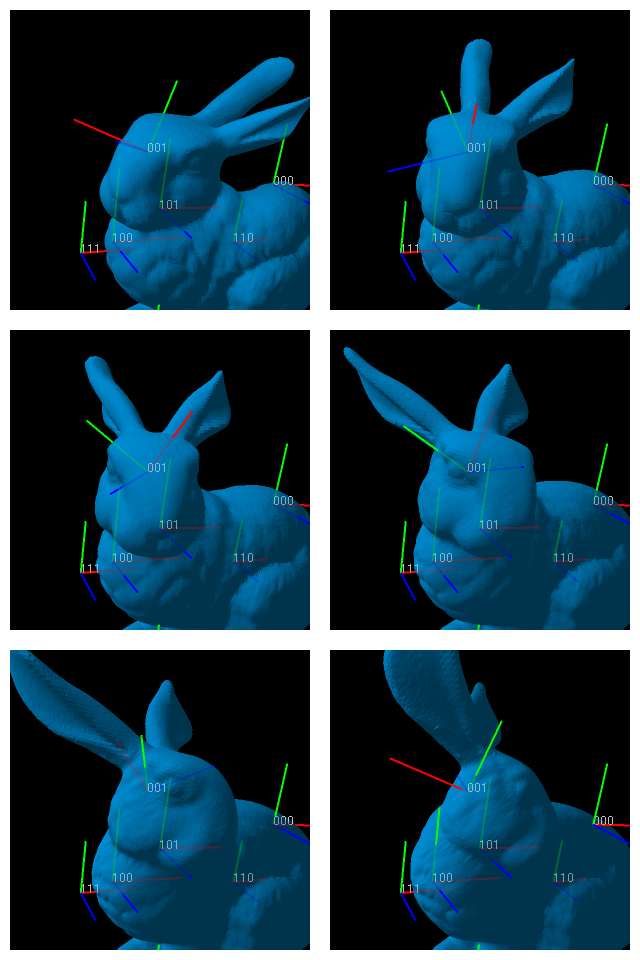
\includegraphics[height=0.8\textheight]{mesh_example}
\caption{\label{fig:meshexample}An example of animating a rabbit's head using key-rotors and an automatically
  assigned mesh.}
\end{figure}

The quality of a mesh deformation technique is ultimately subjective. A simple
example is shown in figure \ref{fig:meshexample}. In this example there were
eight key rotors labelled `000' to `111' in binary. The rotors were moved to
positions within a rabbit model and appropriate weighting and offset-vectors
were assigned using algorithm \ref{alg:meshpoint}. The `001' rotor, which was
positioned within the rabbit's head, was then moved and the results are shown.
The movement is smooth, natural and intuitive.

\begin{figure}[p]
\centering
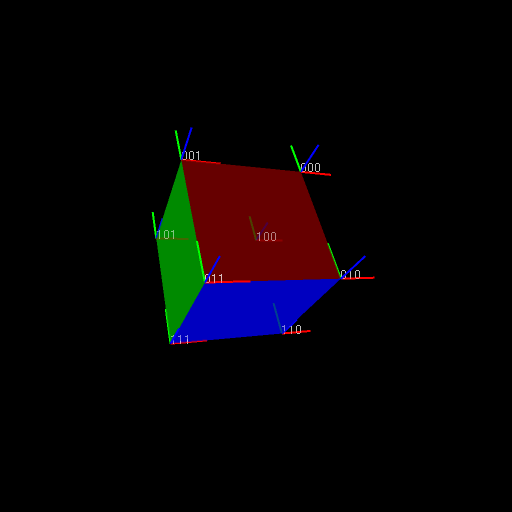
\includegraphics[height=0.37\textheight]{cube_before} \\
\noindent (a) \\ \rule{0pt}{\parskip} \\
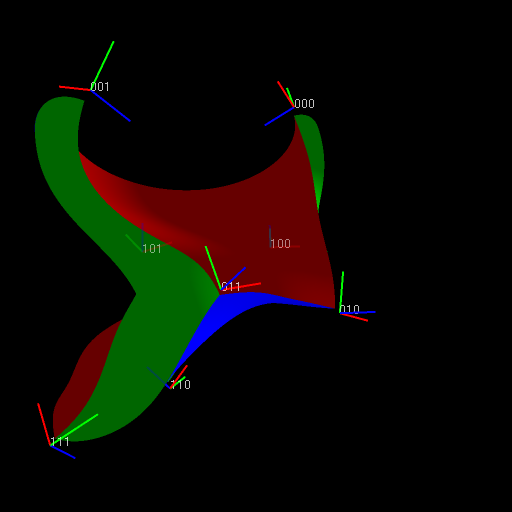
\includegraphics[height=0.37\textheight]{cube_after} \\
\noindent (b) 
\caption{\label{fig:cubeexample}An example of mesh deformation acting on a unit cube.
  (a) Initial key-rotors and automatically assigned mesh. 
  (b) Deformed mesh after movement of key-rotors.} 
\end{figure}

\begin{figure}[p]
\centering
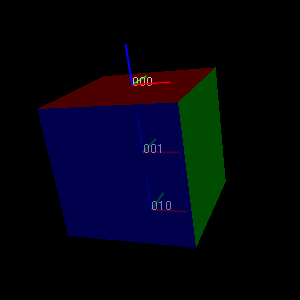
\includegraphics[height=0.37\textheight]{twist_cube_before} \\
\noindent (a) \\ \rule{0pt}{\parskip} \\
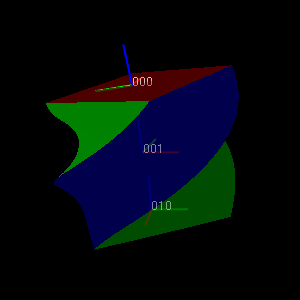
\includegraphics[height=0.37\textheight]{twist_cube_after} \\
\noindent (b) 
\caption{\label{fig:twistcubeexample}An example of twist deformation acting on a unit cube.
  (a) Initial key-rotors and automatically assigned mesh. 
  (b) Twisted mesh after movement of key-rotors.} 
\end{figure}

Figure \ref{fig:cubeexample} shows the natural `plasticine-like' effect the deformation
scheme has on a unit cube with key-rotors initially placed on its corners. In addition to
this figure \ref{fig:twistcubeexample} shows the effect of placing the key rotors along
a central axis and applying opposite rotations at either end. Notice how the cube behaves as
expected and does not collapse in the middle.

\subsection{Performance}

\begin{table}[p]
\centering
\scalebox{0.8}{%
\begin{tabular}{|c|c|c|c|}
\hline                 
 & \multicolumn{2}{c|}{Frames per second} & \\
\hline                 
Polygons & Hardware & Software & Ratio \\
\hline                 
\hline                 
14,406 & 219.10 & 18.81 & 11.65:1\\
20,886 & 160.80 & 12.50 & 12.86:1\\
29,400 & 119.50 & 9.08 & 13.16:1\\       
43,350 & 83.91 & 6.26 & 13.40:1\\
60,000 & 62.13 & 4.65 & 13.36:1\\
\hline                 
\end{tabular}%
\hspace{3ex}
\begin{tabular}{|c|c|c|c|}
\hline                 
 & \multicolumn{2}{c|}{Frames per second} & \\
\hline                 
Polygons & Hardware & Software & Ratio \\
\hline                 
\hline                 
93,750 & 20.42 & 2.89 & 7.07:1\\        
135,000 & 14.20 & 2.07 & 6.86:1\\
240,000 & 8.13 & 1.14 & 7.13:1\\         
372,006 & 5.32 & 0.75 & 7.09:1\\         
-- & -- & -- & -- \\
\hline                 
\end{tabular}
}
\caption{\label{tab:performance}The relative performance, in frames per
second, between the GPU and pure-software mesh deformation implementations.%
}
\end{table}

\begin{figure}[p]
\centering
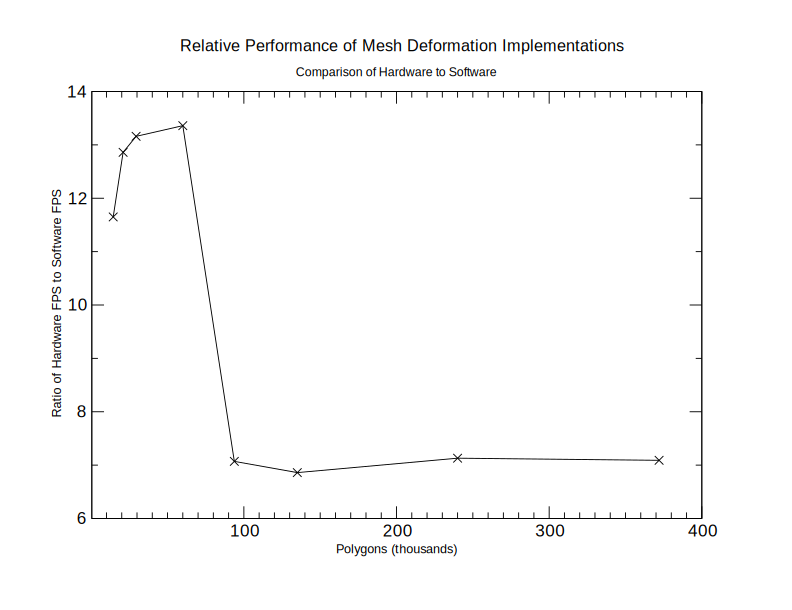
\includegraphics[width=0.9\textwidth]{performance}
\caption{\label{fig:performance}A plot of the ratio between FPS using the
GPU-based implementation and the pure-software implementation.}
\end{figure}

To test the relative performance of software and hardware two implementations
were made, one software and one hardware. Both implemented the same mesh deformation
algorithm as above and both used as near equal, within the intersection of C and
Cg, implementations of the generator exponentiation and rotor application
routines.

The implementations differed most in the use of display lists. To mirror real-world
practises each model in the hardware implementation was uploaded to the graphics
card in a display list since the per-vertex set of $d_{k,i}$ and $p_i$ could
be pre-computed. In the software implementation these were also pre-computed but the
deformed vertices had to be uploaded to the graphics card once-per frame since the
deformation step was done in software.

Table \ref{tab:performance} shows the number of frames per second that could be
displayed with a simple cube model at various different polygon counts. A simple model
was chosen so that the generation, per frame, of un-deformed model vertices in the
software implementation would take as little time as possible being 
algorithmically generated rather than fetched from main memory providing a fairer
test of the speeds of the deformation algorithm. Figure \ref{fig:performance} shows
the ratio of improvement between software and hardware implementations with polygon
count.

\section{Dynamics}

In this section we will develop a simple method for doing dynamics with a sphere
which has been deformed with a set of rotors. We shall show how a simple dynamics example
using such a method may be implemented on the GPU.

Recall that a GPU has two classes of shaders; it has vertex shaders which are applied
per-vertex and fragment shaders which are applied per-pixel. Since, in a typical scene,
one would expect the number of pixels on screen to be very much greater than the number
of vertices, GPUs generally have more parallel fragment shaders than vertex shaders.
If we can re-formulate our solution to use fragment shaders we might expect even
greater performance than simply using the vertex shader.

Algorithms implemented on the fragment shaders have one further 
advantage when compared to those implemented on the vertex shader when one makes use
of the \emph{render to texture} feature on modern graphics cards. Using this feature
rendering can be directed to a texture stored in the graphics card memory rather than the
screen. This feature allows iterative algorithms to be developed.
The concept is simple. A texture is created which stores a set of initial values. 
A square is then rendered with a fragment shader which, for each pixel in the square,
reads the initial value from the texture and outputs the result of the next iteration.
If this square is rendered into the original texture then the result of each iteration
replaces the previous one. This process may be repeated as often as is desired.
In reality there are a few implementation issues. Aside from the API calls required to
setup the render to texture and appropriate projection matrices a significant issue is
that the shader is required to write back to its input which could lead to
concurrency issues. To avoid this one generally uses two textures, an `input' and `output',
which are swapped between each iteration.

\subsection{Collision detection via deformation}

\begin{figure}
\centering
\includegraphics[width=0.8\textwidth]{deformation_scheme}
\caption{\label{fig:deformation_scheme}Given a deformation scheme $\mathcal{D}$ which maps
  our object to the unit sphere we can tell whether a point, $P$, is inside the object by
          testing if the mapped point, $P'$, is inside the sphere.}
\end{figure}

We shall develop a simple example to illustrate this method. In our example we
shall implement an approximate simulation of a cloth falling onto a complex
smooth object. 

To begin with we need a GPU-based simulation of the cloth itself for when
it is moving in space away from the target object. The aim of this example is
to demonstrate complex collision rather than cloth simulation \emph{per se}
and so we choose a very simple ball and spring model; the cloth is composed
of a $N\times M$ grid of masses connected by simple Hookian springs. Formally, 
if we let $P_{i,j}$
be the position vector of the ball in row $i$, column $j$ then the force acting
on it, $F_{i,j}$ is
\[
F_{i,j} = \sum_{\alpha \in \{-1,1\}} \sum_{\beta \in \{-1,1\}} 
b_{i+\alpha, j+\beta} 
\left| P_{i,j} - P_{i+\alpha, j+\beta} \right|
\]
where
\[
b_{i,j} = 
\left\{
\begin{array}{ll}
1 & {\rm ~if~} i \in \{1, \cdots, N\}, j \in \{1, \cdots, M\} \\
0 & {\rm ~otherwise}
\end{array}
\right.
\]
The variation of $P_{i,j}$ over time may then be obtained by numerically
integrating the force twice.

Such simple dynamics are often employed in games where the appearance of
correct physics is often more desirable, if it is faster, than a full
`correct' calculation. We shall use a common game technique %[FIXME:reference]
which may be summarised as `detect and backtrack'.

Suppose a cloth vertex were known to be outside of the target object at time
$t$ and we detect it is to be inside the object at time $t + \Delta t$. 
We stop the simulation and backtrack to time $t + \Delta t - t_{\rm offset}$
with $t_{\rm offset} < \Delta t$ such that the vertex is just touching
the target object. We then use simple surface physics to modify the total
force acting on the vertex to cause reflection, friction or any other 
surface property we may wish. The simulation is then restarted from this point.

We shall discuss the precise implementation of the cloth simulation later but
for the moment we note that the key operation is detecting the interpenetration
of the grid of cloth vertices and the target object and being able to move 
penetrating vertices to the surface of the object.

Our approach is illustrated in figure \ref{fig:deformation_scheme}. We shall
assume some invertible, locally conformal, GA-based deformation scheme
$\mathcal{D}$ which will deform the unit sphere to our target object.  We now
apply the inverse scheme $\mathcal{D}$ to both our target object and the set
of cloth vertices. The target object is mapped to the unit sphere and the set
vertices are mapped to a different set of vertices.  Our penetration test for
vertices is simply to see if its distance from the origin is less than unity.
We can thereby identify all penetrating vertices. Any penetrating vertex can
be corrected simply by moving the deformed vertex to the unit-sphere surface.
If we re-apply the deformation scheme the unity sphere is mapped back to the
target object and the set of corrected vertices is mapped to a set which all
lie outside the target object.

\subsection{A suitable deformation scheme}

We wish our deformation scheme to be locally conformal and, preferably, for the
normal information associated with any point on the target object to be preserved
for lighting and dynamics. Below we preset a simple scheme based upon weighted sums
of pure-rotation generators which fulfils this requirement.

We begin by considering a rotor, $R_i = \exp(B_i)$, representing a rotation around a 
known point $P_i$. Clearly $R_{i,\lambda} = \exp(\lambda B_i)$ is also a pure-rotation
for some scalar $\lambda$. To deform a particular
point representation, $X = F(x)$, using the key-generator $B_i$ we perform the mapping
\[
X \mapsto R_{i,w(X,P_i)}X\tilde{R}_{i,w(X,P_i)}
\]
where $w(A,B)$ is a weighting function with range $[0,1]$. For a simple deformation
scheme we might choose $w(\cdot)$ to be
\[
w(A,B) = \left\{
  \begin{array}{ll}
  1 - d(A,B) &{\rm ~if~} d(A,B) < 1\\
          0 & {\rm ~otherwise}
  \end{array}
  \right.
\]
where $d(A,B)$ is the Euclidean distance metric defined in equation \ref{distance}.
This is of course a linear fall-off. One could easily create non-linear exponential
or sigmoid fall-off which would lead to smoother deformation at the cost of greater
computational complexity.

The effect of the deformation scheme is shown diagrammatically in figure
\ref{fig:weighted_rotor}b. Here four unit lengths are deformed by rotating points
on a set of spherical shells centred on $P_i$. On each spherical shell the deformation
is therefore locally conformal. Normal to the shells the deformation is less so but,
as is often the case in Computer Graphics, the errors introduced by this
may be ignored since they are perceptually slight.

\begin{figure}
\centering
\includegraphics[width=\textwidth]{weighted_rotor}
\caption{\label{fig:weighted_rotor}%
  Diagram illustrating weighted generator deformation around a point $P$. 
          a) Un-deformed state. b) Effect of weighted rotation deformation.
}
\end{figure}

Since we are using position-dependent rotors we can view the deformation not as a point-wise 
deformation scheme but a full local-frame deformation scheme. For example we can represent an
orientation associated with $X$ as a pure-rotation rotor, $R_X$, which is applied to some known
reference orientation. The post-deformation orientation is now
\[
R_X \mapsto R_{i,w(X,P_i)}R_X.
\]
Specifically, if the point $X$ is a mesh vertex with associated normal
$\hat{n} = R_Xe_1\tilde{R}_X$ then we can find the deformed normal, $\hat{n}'$ as
\[
\hat{n}' = R_{i,w(X,P_i)}R_Xe_1\tilde{R}_X\tilde{R}_{i,w(X,P_i)}.
\]

This `frame deformation' property is a key one when it comes to performing perceptually
valid dynamics on deformed objects.

% \subsection{Cloth dynamics}

\subsection{Implementation}

There are two stages to each step of the simulation; firstly the location of
the cloth vertices are updated followed by the detection and correction of
vertices which penetrate the object. For these vertices we perform some basic
surface-physics removing force components normal to the surface and crudely
modelling friction by multiplying the tangential velocity component by some
fixed friction coefficient between 0 and 1.

Both of these steps are performed on the GPU. Unlike the previous example this
simulation required feedback; the output from the simulation had to be fed back
to the input.

% \subsubsection{Cloth simulation}

The first stage in the simulation is the calculation of forces, velocities
and positions for each cloth vertex. 

The location of each cloth vertex was stored in a texture with each pixel in the
texture corresponding to a vertex in the cloth. The red, green and blue
components specified the $x$, $y$ and $z$ co-ordinates respectively.  Many GPUs
only allow for texture components to be in the range $[0, 1]$, effectively
restricting the cloth to the unit cube. This could have been overcome with the
introduction of appropriate scaling constants but newer nVidia GPUs allow for
\emph{float buffers} which remove this restriction and they were used in this
implementation due to their increased accuracy and convenience. A simple vertex shader
could then be used when rendering the cloth to position the vertices according to the
contents of the texture.
In addition to the vertex texture a separate texture was created holding the 
velocity of each cloth vertex in a similar manner. 

To update these textures we made use of \emph{render to texture} support in newer GPUs
where pixel and vertex shaders can be used to render images, not to screen, but to
a particular texture. By rendering a single quad (or two triangles) into a texture
we could invoke the pixel shader for each texel.

GPUs cannot access the texture they are rendering into within pixel shaders for
concurrency reasons and hence two pairs of textures were maintained, one pair
for the velocities and one pair for the vertex positions. At each step one
member of the pair would reflect the `current state' and the other would be
written into representing the `new state'. At the end of the simulation step
their r\^oles would be reversed.

% \subsubsection{Deformation}

\begin{figure}[p]
\centering
\scalebox{0.7}{
\begin{minipage}{\textwidth}
\singlespacing
\lstinputlisting[language=c]{calcForces.cg}
\end{minipage}}
\caption{\label{fig:calcForces}The pixel shader for summing the forces on the cloth vertices
and removing normal components of velocity.}
\end{figure}

\begin{figure}[p]
\centering
\scalebox{0.7}{
\begin{minipage}{\textwidth}
\singlespacing
\lstinputlisting[language=c]{calcVertices.cg}
\end{minipage}}
\caption{\label{fig:calcVertices}The pixel shader used to update the vertex position and
correct for penetration.}
\end{figure}

The first part of figure \ref{fig:calcForces} shows the shader used to sum forces. The force
on each vertex is calculated as the sum of forces due to Hookian springs which connect it
to its immediate neighbours. The integration of force over time to give velocity
is simply Euclid's method due to its ease of implementation and compactness; space is a premium
in shaders.

The first part of figure \ref{fig:calcVertices} shows the shader used to update vertex positions.
Again the velocity is integrated by simple summing to make the shader small and fast.

\begin{figure}[p]
\centering
\scalebox{0.7}{
\begin{minipage}{\textwidth}
\singlespacing
\lstinputlisting[language=c]{map.cg}
\end{minipage}}
\caption{\label{fig:map}The vertex shader utility functions for mapping to and
  from a rotor-deformed space.}
\end{figure}

The second part of the simulation takes place after deformation such that the
target object becomes the unit sphere. In figure \ref{fig:calcVertices} the new
vertex position is simply moved so that it does not penetrate the object. In
figure \ref{fig:calcForces} some basic surface physics is performed removing
components of velocity into the object and attenuating tangential components to
simulate friction. 

Both shaders use a Cg implementation of the deformation scheme which is
implemented in figure \ref{fig:map}. Here the components of each key-generator
are stored in a texture which is used to deform any vertex passed to the
function.

\subsubsection{Results}

Figure \ref{fig:cloth_montage} shows a selection of scenes from the final demo.
You can see the central object which is a unit-sphere which has been deformed
by 4 key-generators with linear fall-off. The cloth simulation is then allowed
to fall on the object and slides off. All of this is performed on the GPU in
real-time (50 frames per second) for a 1024-vertex cloth model.

\begin{figure}[p]
\centering
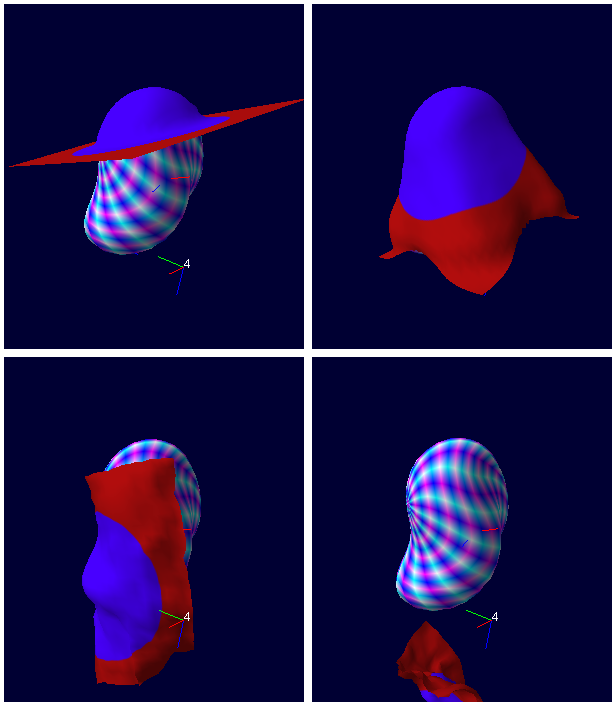
\includegraphics[width=\textwidth]{cloth_montage}
\caption{\label{fig:cloth_montage}%
  A selection of scenes from the penetration demo showing the
  simulation of a simple cloth model on the surface of a deformed
  sphere.
}
\end{figure}

